% !TeX root = ../main.tex

\addchap{Appendix} \label{chapter:appendix}

\refstepcounter{chapter} 
\section{Images}

\begin{figure}[h!tb]
\centering
\begin{subfigure}{1.0\textwidth}
  \centering
  \adjincludegraphics[width=1.0\linewidth,trim={0 0 0 0},clip]{figures/ds/ucf_train_full.png}
  \caption{Training set}
  \label{fig:ucf_train_full}
  \vspace{.1cm}
\end{subfigure}
\caption[UCF-101 Full Image Samples]{Randomly chosen and rescaled clip samples of size $160 \times 120$ from the UCF-101 dataset. There is only a very small portion of motion to see between one frame to the next, because the videos have a frame rate of \num{25} FPS.\\
\textit{(continues on next page)}}
\label{fig:ucf_full}
\end{figure}



\begin{figure}[h!tb]
\ContinuedFloat % continue from previous page
\centering
\begin{subfigure}{1.0\textwidth}
  \centering
  \adjincludegraphics[width=1.0\linewidth,trim={0 0 0 0},clip]{figures/ds/ucf_valid_full.png}
  \caption{Validation set}
  \label{fig:ucf_valid_full}
  \vspace{.1cm}
\end{subfigure}
\begin{subfigure}{1.0\textwidth}
  \centering
  \adjincludegraphics[width=1.0\linewidth,trim={0 0 0 0},clip]{figures/ds/ucf_test_full.png}
  \caption{Test set}
  \label{fig:ucf_test_full}
\end{subfigure}
\caption*{}
\end{figure}







\begin{figure}[h!tb]
\centering
\begin{subfigure}{1.0\textwidth}
  \centering
  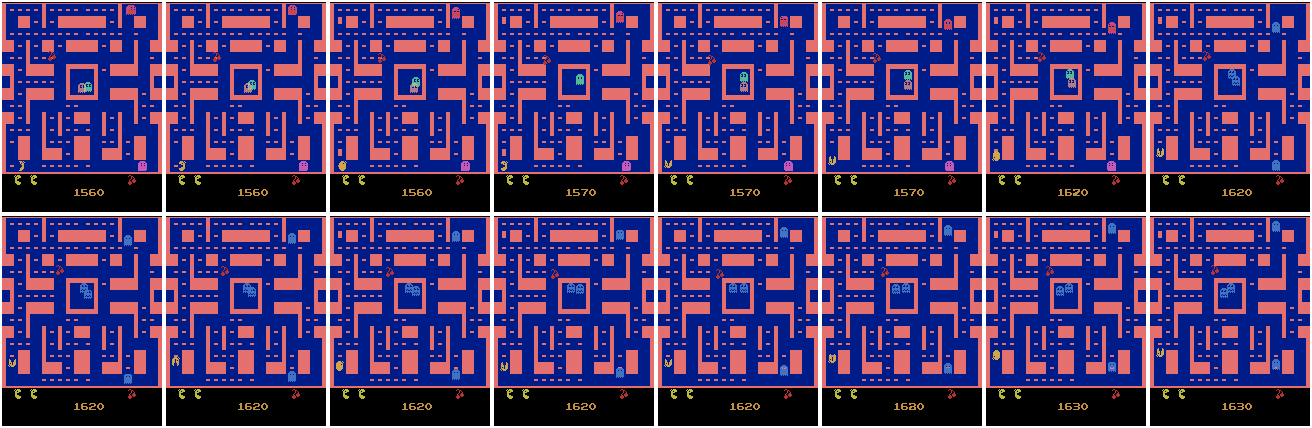
\includegraphics[width=1.0\linewidth]{figures/ds/pac_train_full.png}
  \caption{Training set}
  \label{fig:pac_train_full}
  \vspace{.1cm}
\end{subfigure}
\begin{subfigure}{1.0\textwidth}
  \centering
  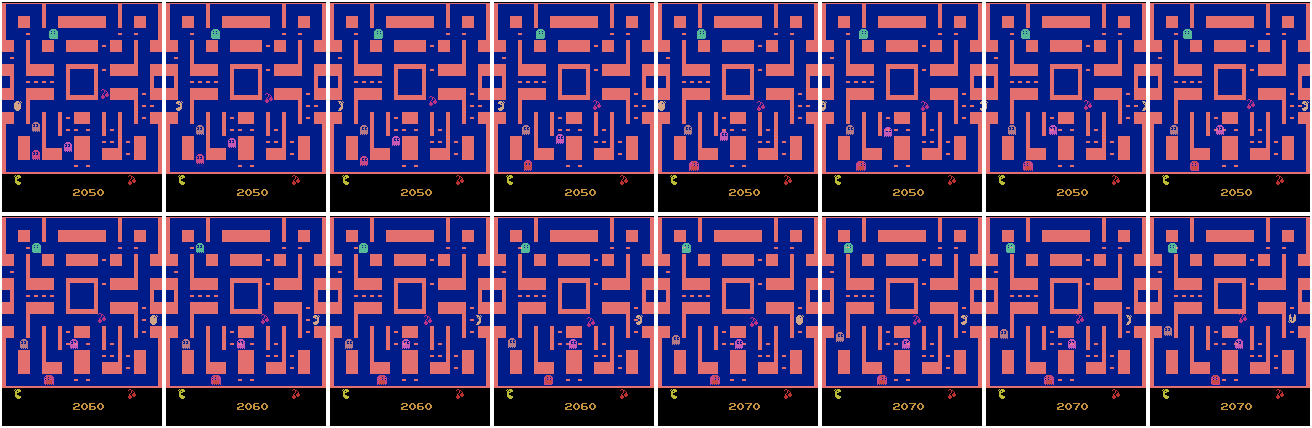
\includegraphics[width=1.0\linewidth]{figures/ds/pac_valid_full.png}
  \caption{Validation set}
  \label{fig:pac_valid_full}
  \vspace{.1cm}
\end{subfigure}
\begin{subfigure}{1.0\textwidth}
  \centering
  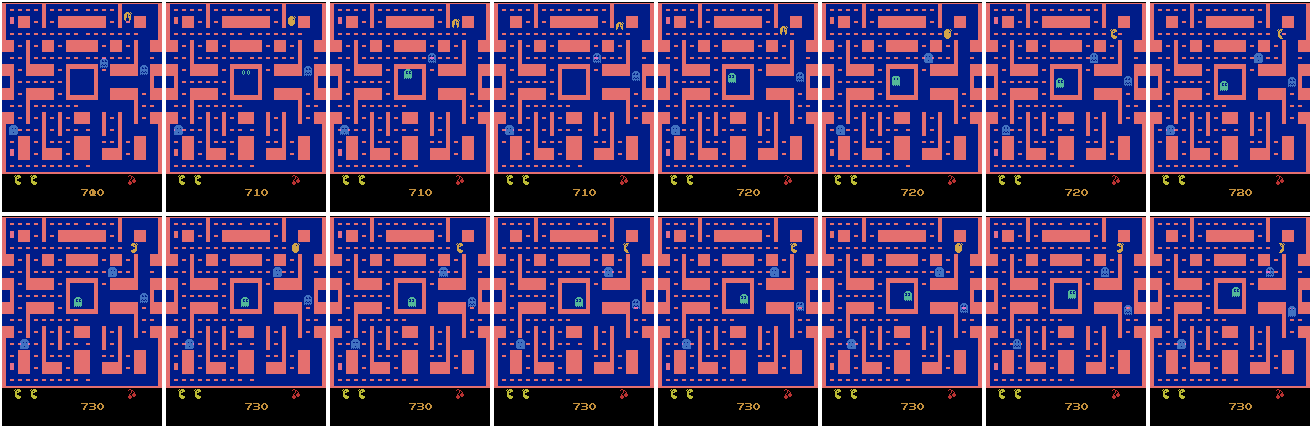
\includegraphics[width=1.0\linewidth]{figures/ds/pac_test_full.png}
  \caption{Test set}
  \label{fig:pac_test_full}
\end{subfigure}
\caption[MsPacman Full Image Samples]{Exemplary sequences of game recordings from MsPacman dataset that have been samples randomly from the different splits. Each shown clip has a length of \num{16} frames of size $160 \times 210$.}
\label{fig:pacman_full}
\end{figure}



\clearpage
%\refstepcounter{chapter} 
\section{Code Listings}

\begin{figure}[h!tb]
  \begin{tabular}{c}
  \begin{lstlisting}[language=Python]
import tensorflow as tf
import tensorlight as tl
from tf.contrib.layers import *

class ConvAutoencoderModel(tl.model.AbstractModel):    
  def __init__(self, weight_decay=0.0):
    super(ConvAutoencoderModel, self).__init__(weight_decay)
        
  @tt.utils.attr.override
  def inference(self, inputs, targets, feeds, is_train, device_scope, memory_device):
    with tf.variable_scope("Encoder"):
      conv1 = tl.network.conv2d("Conv1", inputs, 4, (5, 5), (2, 2),
                                   weight_init=xavier_initializer_conv2d(),
                                   regularizer=l2_regularizer(self.weight_decay),
                                   activation=tf.nn.relu)
      conv1_bn = batch_norm(conv1, is_training=is_train, scope="conv1_bn")
      conv2 = tl.network.conv2d("Conv2", conv1_bn, 8, (3, 3), (2, 2),
                                   weight_init=xavier_initializer_conv2d(),
                                   regularizer=l2_regularizer(self.weight_decay),
                                   activation=tf.nn.relu)
      conv2_bn = batch_norm(conv2, is_training=is_train, scope="conv2_bn")
      learned_rep = conv2_bn
    with tf.variable_scope("Decoder"):
      convt = tl.network.conv2d_transpose("Convt1", learned_rep, 4, (3, 3), (2, 2),
                                              weight_init=tl.init.bilinear_initializer(),
                                              regularizer=l2_regularizer(self.weight_decay),
                                              activation=tf.nn.relu)
      convt_bn = batch_norm(convt, is_training=is_train, scope="convt_bn")
      return tl.network.conv2d_transpose("Convt2", convt_bn, 1, (5, 5), (2, 2),
                                              weight_init=tl.init.bilinear_initializer(), 
                                              regularizer=l2_regularizer(self.weight_decay),
                                              activation=tf.nn.sigmoid)
    
  @tt.utils.attr.override
  def loss(self, predictions, targets, device_scope):
    return tl.loss.bce(predictions, targets) + tl.loss.mgdl(predictions, targets)
    
  @tt.utils.attr.override
  def evaluation(self, predictions, targets, device_scope):
    psnr = tl.image.psnr(predictions, targets)
    sharpdiff = tl.image.sharp_diff(predictions, targets)
    ssim = tl.image.ssim(predictions, targets)
    return {"psnr": psnr, "sharpdiff": sharpdiff, "ssim": ssim}
  \end{lstlisting}
  \end{tabular}
  \caption[Listing: Convolutional Autoencoder]{An example implementation of a convolutional autoencoder model, have an encoder and decoder with two layers each.}\label{code:model}
\end{figure}





